\documentclass[LaTeX2e,10pt,aspectratio=169]{beamer}
\setbeamertemplate{navigation symbols}{}
\usefonttheme[onlymath]{serif}

\usepackage{tikz}

\usetikzlibrary{fit,positioning}
\tikzstyle{every picture}+=[remember picture]

\begin{document}

\bgroup
\setbeamercolor{background canvas}{bg=white}
\begin{frame}[plain]{}
	\begin{tikzpicture}[
    node distance = 7mm and -3mm,
every node/.style = {draw=black, rounded corners, fill=gray!30, 
                     minimum width=2cm, minimum height=0.5cm,
                     align=center}
                        ]
\node (scarce) {(1)};

\node (inpainted)[right=30mm of scarce]{(2)}; 

\node (target)  [below=10mm of inpainted.south] {(3) 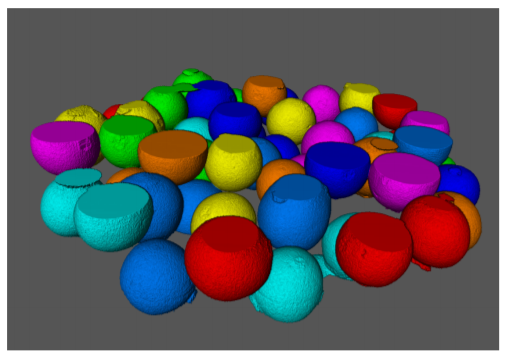
\includegraphics[width=0.2\textwidth]{sophia beads.png}};

\node (detRes)  [below right=17mm and 15mm of inpainted.east] {True or False value};

\draw[->] (scarce) to node {Generator} (inpainted) ;
\draw[->] (inpainted) to node {Discriminator} (detRes) ;
\draw[->] (target) to node {Discriminator} (detRes) ;

\end{tikzpicture}
\end{frame}
\egroup


\end{document}